\documentclass[14pt]{matmex-diploma}

\begin{document}

\filltitle{ru}{
    chair              = {Математическое обеспечение и администрирование информационных систем\\Кафедра информационно-аналитических систем},
    title              = {Автоматическая типизация горных пород},
    type               = {coursework},
    position           = {студента},
    group              = 341,
    author             = {Смирнов Александр Львович},
    supervisorPosition = {ст. преп.},
    supervisor         = {Смирнов М.\,Н.},
    reviewerPosition   = {доцент},
    reviewer           = {Графеева Н.\,Г.},
}

\maketitle

\tableofcontents


\section*{Введение}

    Существует множество способов разведки нефтяных месторождений. Один из них — разведка буром: во время бурения аккуратно извлекают керн — цилиндрические столбики породы, по которым ясно видно, как залегают пласты. Полученные образцы позволяют обнаружить породы-коллекторы, оценить их емкостные и фильтрационные свойства.
    
    \subsection*{Что такое керн}
    
        Керн — цилиндрический монолит горной породы, получаемый путём кольцевого разрушения забоя скважин при бурении.
        
        \begin{figure}[h]
            \label{керн}
            \centering
            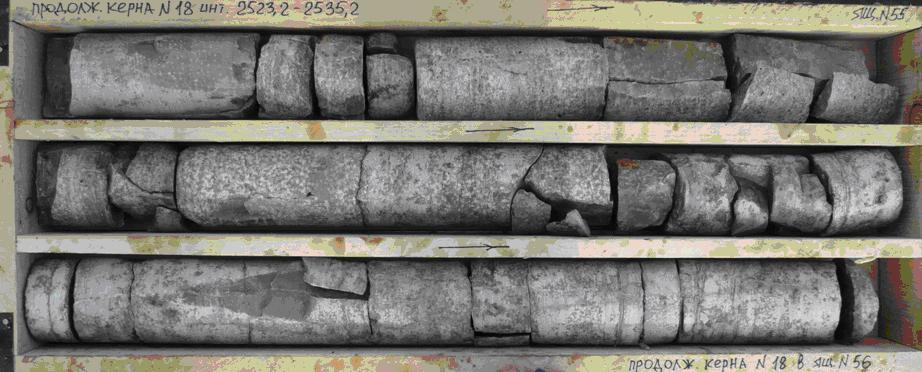
\includegraphics[scale=0.5]{images/kern.jpg}
            \caption{Пример керна}
        \end{figure}
        
        К сохранности и качеству керна предъявляются требования, обеспечивающие достоверность сведений о составе и строении вскрытых скважиной горной породы и полезных ископаемых. Сохранность керна оценивается его линейным (или объёмным) выходом — процентным отношением суммарной длины (или фактической массы) поднятого керна к длине пробуренного интервала (или расчётной массе для пробуренного интервала) скважины.
        
        В дальнейшем керн исследуется и анализируется (химический, спектральный, петрографический и другие анализы) в лаборатории с помощью различных методов и на различном оборудовании, в зависимости от того, какие данные должны быть получены.
        
        Выход керна по руде обычно колеблется от 50 до 80\%. В плотных и однородных рудах и породах он повышается до 100\%. В мягких и сильно трещиноватых рудах выход керна иногда снижается до нуля. При отсутствии или малом выходе керна в пробу поступает шлам, вследствие чего качество опробования значительно снижается. Учитывая это, следует добиваться максимального выхода бурового керна.
        
        При опробовании массивных и вкрапленных руд большой мощности применяется секционный отбор проб с длиной керна отдельной пробы 1, 2 или 3 метра, а иногда 5 метров в соответствии с методами предстоящей эксплуатации.
        
        Описание разреза начинается с общего осмотра керна (или его части) и уточнения его местоположения в разрезе скважины. Керн, поднятый и очищенный от бурового раствора, укладывают в специальные керновые ящики, изготовленные из дерева и разделенные на продольные секции. После этого проводятся исследования состава, выделение маркирующих слоёв и прочее.
        
    \subsection*{Исследование керна}
    
        Изучение нефтегазоносных скважин по керну имеет свои специфические особенности. Они заключаются в том, что по керну скважин получают в основном геологическую информацию, связанную с закономерностями вертикального строения разрезов (последовательность и характер напластования, мощность слоев, литологический состав отложений, текстурно-структурные особенности пород и т.д.).
        
        Кроме того, отбор керна в скважинах осуществляется не полностью, поэтому полученные сведения могут носить обрывочный характер и требуют глубокого анализа строения разрезов, вскрытых ранее пробуренными скважинами, и привлечения данных геофизических исследований.
        
        Осадочные толщи имеют слоистое (часто ритмичное) строение и представляют многократное и разномасштабное повторение (чередование) пород. Поэтому при осмотре и описании керновых колонок, прежде всего, выделяются слои – геологические тела, имеющие существенно однородный литологический состав (часто одинаковую окраску), обладающие ясно выраженными подошвой и кровлей и значительной толщиной (мощностью).
        
    \subsection*{Определение наличия нефти}
    
        Фотографии керна в ультрафиолетовом свете (\ref{UV}) позволяют выделить в разрезе нефтенасыщенные участки, выявить текстурные характеристики, связанные с особенностями условий осадконакопления пород. Нефтенасыщенные интервалы керна светятся в ультрафиолетовом свете в спектре от голубого до буровато-оранжевого цвета. Чем выше плотность углеводородов и насыщенность ими пород, тем больше желтых, оранжевых и коричневых цветов. \cite{paper:kern}
        
        \begin{figure}[h]
            \centering
            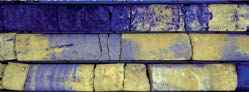
\includegraphics[scale=1]{images/UV.png}
            \caption{Фотографии керна в ультрафиолетовом свете. Неравномерное желтое свечение – неравномерно нефтенасыщенные песчаник.}
            \label{UV}
        \end{figure}        
        
        Нефтепроявления могут заключаться в выходах жидкой нефти и подъеме нефтесодержащих пород, в примазках нефти по трещинам в породах, в тонких пленках нефти на воде и т.д. Нефть может вытекать непосредственно из коренных пород, из наносов; может скапливаться в виде толстых плёнок на поверхности воды более или менее далеко от места выхода нефтеносных пород на дневную поверхность и т.д.
        
        При изучении керна иногда можно наблюдать налеты и примазки нефтяных компонентов на стенках трещин. Обычно они темноокрашенные, так как представляют собой остаточные, окисленные компоненты мигрировавших через породу нефтяных флюидов: асфальтеновых и смолисто-асфальтеновых фракций. Легкие и средние компоненты (бесцветные и светлоокрашенные) даже при интенсивном нефтяном запахе породы остаются невидимыми.
        
        Нефтесодержащие породы узнаются или сразу по цвету и запаху, если они сильно пропитаны нефтью, или после проверочных испытаний. Нефть может быть распределена в породе (например, в песчанике) равномерно или, чаще, неравномерно. В этом случае необходимо изучить характер ее распределения в зависимости от состава, структуры и текстуры.
        
        Неравномерные признаки нефтенасыщения в виде «пятнистости» по всему интервалу керна чаще всего наблюдаются в переходных зонах, ближе к водонефтяным контактам или в неоднородном пласте-коллекторе с резкой изменчивостью ёмкостно-фильтрационных свойств. В этом случае необходимо детально изучить весь интервал керна на нефтенасыщенность. \cite{paper:oil}
        
    \subsection*{Проблема}
        
        Информация о керне описывается послойно: один слой - один тип породы.
        
        В какой-то момент времени геологи поняли, что стоит детализировать описание пород: нарезали слои на фрагменты по изображениям с шагом до 1 метра и сделали для таких изображений экспертную разметку (разметка делалась несколькими экспертами, мнение которых могло не совпадать друг с другом).
        
        Недавно геологи задумались о том, что можно размечать изображения керна с большей точностью, что позволит создавать более точные модели пластов.


\section{Цели работы}

    Целью данной работы является получение описания керна на основе выборки фотографий. Описание должно включать в себя:
    
    \begin{itemize}
        \item Тип породы с точностью до 20 см. 
        \item Карбонатность с точностью до 10 см.
        \item Нефтенасыщенность с точностью до 10 см.
        \item Разрушенность с точностью до 5 см.
    \end{itemize}
    
    Также целью работы является написание удобной для пользователя обёртки над полученным решением для последующего использования.


\section{Постановка задачи}

    Для достижения приведённых целей были поставлены следующие задачи:
    
    \begin{itemize}
        \item Произвести разведочный анализ предоставленных данных
        \item Ознакомиться с возможными решениями
        \item Реализовать решения и найти лучшие
        \item Сравнить результаты с уже имеющимися у заказчика
        \item Создать оболочку для удобного использования решения
    \end{itemize}    
    

\section{Исходные данные}

    


\section{Решение}

    \subsection{Обзор вариантов}
    



\section*{Заключение}


\setmonofont[Mapping=tex-text]{CMU Typewriter Text}
\bibliographystyle{ugost2008ls}
\bibliography{diploma.bib}
\end{document}